\section{Perspective projections}

Parallel projections maintain the apparent size of an object regardless of its distance from the observer, making them commonly employed in technical drawings. 
On the other hand, perspective projections depict objects with varying sizes based on their distance from the projection plane, making them better suited for immersive visualizations.

The magnification effect occurs because all projection rays converge at a single point.
For simplicity, let's consider a side view where the projection plane is reduced to a line.

Rays intersect the projection plane at varying points based on the object's distance. 
Comparing segments from objects of equal size, but different distances reveals that closer objects to the plane exhibit larger projections.

A point with coordinates ($x, y, z$) in space is projected onto the plane, resulting in a point with Normalized Screen Coordinates ($x_s, y_s, z_s$), where $z_s$ is necessary to order points based on their distance from the viewer, as in the case of parallel projections. 
Initially, we'll concentrate on $y_s$, followed by $x_s$, and finally on $z_s$.
Specifically, when focusing on the $y$-axis, we can calculate the normalized screen coordinate $y_s$ as the projection of the vertical component of the point ($x, y, z$) onto the plane.
\begin{figure}[H]
    \centering
    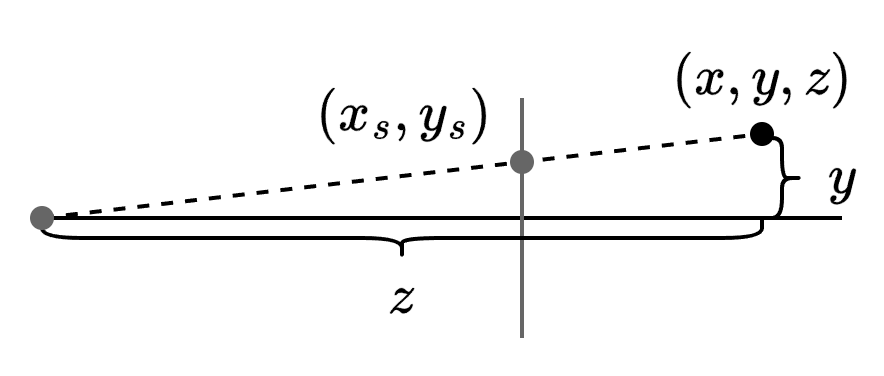
\includegraphics[width=0.5\linewidth]{images/perp.png}
    \caption{Perspective projection with respect to $y$-axis}
\end{figure}
For ease of computation, we place the center of projection at the origin ($0, 0, 0$). 
The projection plane is positioned at a distance d along the $z$-axis from the projection center. 
Examining the image below, we notice two similar triangles: $ABC$ and $ADE$. 
Here, $y_s$ represents the height of the smaller triangle, while the world coordinate $y$ represents the height of the larger one.
\begin{figure}[H]
    \centering
    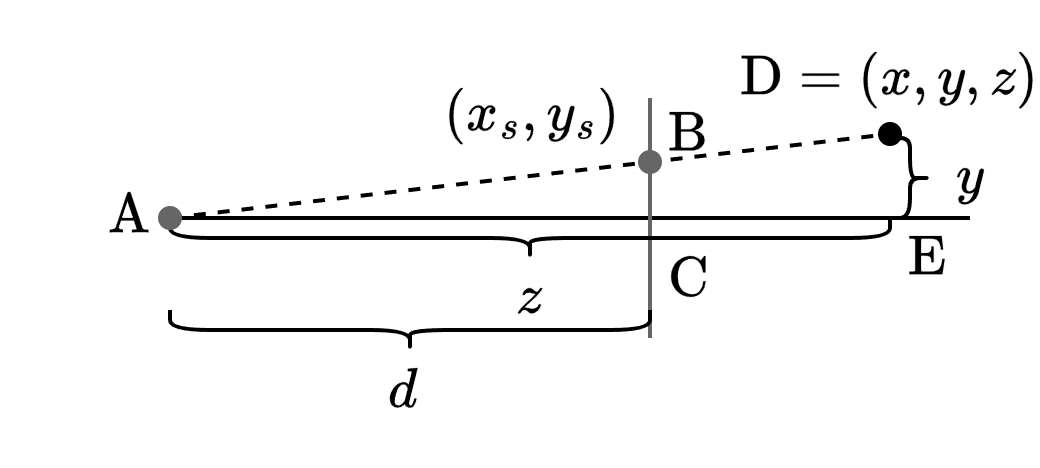
\includegraphics[width=0.5\linewidth]{images/perp1.png}
    \caption{Perspective projection with respect to $y$-axis with triangles}
\end{figure}
Due to the similarity of the two triangles, there exists a linear relationship among the lengths of their edges. 
Specifically, we have:
\[y_s=\dfrac{d\cdot y}{z}\]
The same reasoning applies to $x_s$ as well:
\[x_s=\dfrac{d\cdot x}{z}\]

\paragraph*{Focal length}
Parameter $d$ signifies the distance between the center of projection and the projection plane. 
It can be utilized to simulate the focal length of a camera lens. 
Notably, adjusting $d$ results in a zoom effect.

A short $d$ corresponds to a wide-lens effect: it accentuates the distances of objects from the plane. 
Additionally, it enables the capture of a larger number of objects in the view, resulting in smaller objects in the images.

A large $d$ corresponds to a tele-lens effect, minimizing the differences in size for objects at various distances. 
It also decreases the number of objects visible in the scene, resulting in enlarged views.

Parallel (orthographic) projections can be derived from perspective projections as $d$ approaches infinity.

\paragraph*{Perspective projections matrices}
With the aid of homogeneous coordinates, perspective projections can also be achieved through a matrix-vector product. 
It's important to recognize that the world coordinate system under consideration is oriented oppositely along the $z$-axis, meaning the $z$-coordinates are negative: 
\[x_s=\dfrac{d\cdot x}{-z}\qquad y_s=\dfrac{d\cdot y}{-z}\]
The formula under consideration requires a sign change to accommodate the actual direction of the $z$-axis.
In Vulkan, the $y$-axis should also be mirrored, but it will be easier to perform this in a separate final step.
The projection matrix for perspective, with center in the origin and projection plane at distance $d$ on the $z$-axis, can be defined as:
\[P_{persp}=\begin{bmatrix}
    d & 0 & 0 & 0 \\
    0 & d & 0 & 0 \\
    0 & 0 & d & 0 \\
    0 & 0 & -1 & 0 \\
\end{bmatrix}\]
Note that the last row of this transform matrix is no longer equal to $\begin{bmatrix} 0 & 0 & 0 & 1 \end{bmatrix}$. 
This also makes the product of matrix $P_{persp}$ with a homogeneous coordinate resulting in a vector with component $w \neq 1$.


The previous method comes with a drawback: the $z$ component of the resulting Cartesian coordinate is consistently $-d$, resulting in the loss of information regarding the distance from the projection plane. 
Consequently, it is not possible to define accurate 3D Normalized Screen Coordinates with a $z_s$ component that accurately represents the point's distance from the view plane.
Since $z_s$ is only utilized for sorting primitives, it suffices to insert an element equal to $1$ in the third row of the fourth column of the matrix to achieve a $z_s$ component that consistently varies with the distance of the point: 
\[P_{persp}=\begin{bmatrix}
    d & 0 & 0 & 0 \\
    0 & d & 0 & 0 \\
    0 & 0 & d & 1 \\
    0 & 0 & -1 & 0 \\
\end{bmatrix}\]

Similar to parallel projections, the visible area of the 3D world corresponds to normalized screen coordinates within the range $[-1, +1]$ for $x$ and $y$, and $[0, 1]$ for $z$. 
Additional transforms are then applied to ensure this range corresponds to the specific area of the world we aim to display.
Let $n$ represent the distance from the origin to the near plane.
We denote $l$, $r$, $t$, and $b$ as the coordinates of the left, right, top, and bottom edges of the projection plane in world space at the near plane.
Lastly, $f$ denotes the distance from the origin to the far plane.
It's important to note that, because of perspective, the coordinates of the screen borders at the far plane differ from those at the near plane. 
Consequently, the visible area is not a box but rather a frustum.
Additionally, it's worth noting that the coordinates of the screen borders don't necessarily need to be symmetric. 
This flexibility can be utilized to calculate shifted viewports, enabling the sharing of a projection over two adjacent screens, for instance.
Given that the coordinates of the screen border are defined at the near plane, the value of $n$ corresponds to the distance of the projection plane, denoted as $d$.
It's important to emphasize that for perspective projections, $n$ must be greater than $0$.
The initial step involves writing the previously introduced projection matrix while substituting $d$ with $n$:
\[U_{persp}=\begin{bmatrix}
    n & 0 & 0 & 0 \\
    0 & n & 0 & 0 \\
    0 & 0 & n & 1 \\
    0 & 0 & -1 & 0 \\
\end{bmatrix}\]
To derive Normalized Screen Coordinates, additional transformations need to be sequentially applied.
Starting with the given values of $l$, $r$, $t$, and $b$ at the near plane, we first calculate the projections of the top-left and bottom-right corners at the near plane.
\[\begin{bmatrix}
    n & 0 & 0 & 0 \\
    0 & n & 0 & 0 \\
    0 & 0 & n & 1 \\
    0 & 0 & -1 & 0 \\
\end{bmatrix} 
\begin{bmatrix}
    l \\
    t \\
    -n \\
    1 \\
\end{bmatrix} =
\begin{bmatrix}
    nl \\
    nt \\
    -n^2 + 1\\
    n \\
\end{bmatrix}=
\begin{bmatrix}
    l \\
    t \\
    -n + \frac{1}{n}\\
    1 \\
\end{bmatrix}\]
\[\begin{bmatrix}
    n & 0 & 0 & 0 \\
    0 & n & 0 & 0 \\
    0 & 0 & n & 1 \\
    0 & 0 & -1 & 0 \\
\end{bmatrix} 
\begin{bmatrix}
    r \\
    b \\
    -n \\
    1 \\
\end{bmatrix} =
\begin{bmatrix}
    nr \\
    nb \\
    -n^2 + 1\\
    n \\
\end{bmatrix}=
\begin{bmatrix}
    r \\
    b \\
    -n + \frac{1}{n}\\
    1 \\
\end{bmatrix}\]
Additionally, we need to calculate the projected coordinates of a point at the far plane ($z=-f$) to establish the appropriate normalization for the $z$-axis.
\[\begin{bmatrix}
    n & 0 & 0 & 0 \\
    0 & n & 0 & 0 \\
    0 & 0 & n & 1 \\
    0 & 0 & -1 & 0 \\
\end{bmatrix} 
\begin{bmatrix}
    x \\
    y \\
    -f \\
    1 \\
\end{bmatrix} =
\begin{bmatrix}
    nx\\
    ny \\
    -n^f + 1\\
    f \\
\end{bmatrix}=
\begin{bmatrix}
    \frac{n \cdot x}{f} \\
    \frac{n \cdot y}{f} \\
    \frac{1}{f}-1\\
    1 \\
\end{bmatrix}\]
We have also that: 
\[T_{persp}= \begin{bmatrix}
    1 & 0 & 0 & -\frac{r+l}{2} \\
    0 & 1 & 0 & -\frac{t+b}{2} \\
    0 & 0 & 1 & -\left(\frac{1}{n}-n\right) \\
    0 & 0 & 0 & 1 \\
\end{bmatrix} \qquad
S_{persp}= \begin{bmatrix}
    \frac{2}{r-l} & 0 & 0 & 0 \\
    0 & \frac{2}{t-b} & 0 & 0 \\
    0 & 0 & \frac{nf}{n-f} & 0 \\
    0 & 0 & 0 & 1 \\
\end{bmatrix} \qquad
M_{persp}= \begin{bmatrix}
    1 & 0 & 0 & 0 \\
    0 & -1 & 0 & 0 \\
    0 & 0 & 1 & 0 \\
    0 & 0 & 0 & 1 \\
\end{bmatrix}\]
Combining all the elements, we obtain; 
\[P_{persp}=\begin{bmatrix}
    \frac{2n}{r-l} & 0 & \frac{r+l}{r-l} & 0 \\
    0 & \frac{2n}{b-t} & \frac{t+b}{b-t} & 0 \\
    0 & 0 & \frac{f}{n-f} & \frac{nf}{n-f} \\
    0 & 0 & -1 & 0 \\
\end{bmatrix}\]
As for parallel projection, the values $l$, $r$, $t$ and $b$ must be consistent with the aspect ratio $a$ of the monitor.
\[l-r=a\cdot(t-b)\]

\paragraph*{Camera}
In many scenarios, a set of parameters resembling those found in a camera is employed. 
These typically include the distances $n$ and $f$ of the near and far planes, the angle $\Theta$ at the top of the frustum (referred to as the field of view or $fov_y$) along the $y$-axis, and the aspect ratio $a$ of the screen.
From the previous definitions we have:
\[t=n\tan\dfrac{\Theta}{2} \qquad b=-n\tan\dfrac{\Theta}{2} \qquad l=-a \cdot n\tan\dfrac{\Theta}{2} \qquad r=a \cdot n\tan\dfrac{\Theta}{2}\]
Plugging the values $l$, $r$, $t$ and $b$ in the $P_{persp}$ matrix we obtain:
\[P_{persp}=\begin{bmatrix}
    \frac{1}{a\cdot \frac{\Theta}{2}} & 0 & 0 & 0 \\
    0 & -\frac{1}{\frac{\Theta}{2}} & 0 & 0 \\
    0 & 0 & \frac{f}{n-f} & \frac{nf}{n-f} \\
    0 & 0 & -1 & 0 \\
\end{bmatrix}\]

\paragraph*{Perspective projections in GLM}
GLM provides the \texttt{frustum ()} function for computing the perspective projection matrix, defining the boundaries of the visible region:
\begin{verbatim}
glm::mat4 Port = glm::frustum(l, r, b, t, n, f);
\end{verbatim}
Here, $l$, $r$, $b$, $t$, $n$, $f$ represent the left, right, bottom, top, near, and far boundaries in world coordinates, respectively.

The \texttt{perspective ()} function computes the perspective projection matrix based on the field of view ($fov$) and aspect ratio ($a$):
\begin{verbatim}
glm::mat4 Port = glm::perspective(fov, a, n, f);
\end{verbatim}
Where $fov$, $a$, $n$, and $f$ denote the vertical field of view, aspect ratio, near plane distance, and far plane distance, respectively.

As for the \texttt{ortho ()} function, originally designed for OpenGL, adjustments are necessary for Vulkan compatibility. 
To achieve this, the following steps are required: 
\begin{verbatim}
#define GLM_FORCE_DEPTH_ZERO_TO_ONE

M2glm = glm::scale(glm::mat4(1.0), glm::vec3(1,-1,1)) * 
        glm::frustum(l, r, b, t, n, f);
M1glm = glm::perspective(fovy, a, n, f);
M1glm[1][1] *= -1;
\end{verbatim}

